\section{基本性能优化：冒险、前递、暂停与冲刷}
\label{sec:04-processor-core-05}

\subsection{从“数据相关”走到“这一拍拿不到数据”}

考虑两条相邻指令：\texttt{addi x1, x0, 5} 与 \texttt{add x2, x1, x1}。
第一条生成 x1，第二条读取 x1，二者存在写后读相关（RAW）。
在本例流水线中，第二条到达 ID 时，第一条还没有到 WB，寄存器堆里仍然是旧 x1。
但“寄存器堆尚未更新”并不等于“芯片内没有正确结果”：第一条的 ALU 已经能够在 EX 末产生 5。
前递就是把这个尚未正式写回的值，送到真正需要它的位置。

因此应把两个概念分开：\textbf{数据相关是指令序列的属性，数据冒险是当前实现的时序约束。}
同一组相关指令，在单周期实现中可能不用处理，在不同分级或存储器时序的流水线中可能需要不同的暂停。
分析时总是先问“生产者何时得到数据”和“消费者在哪一级使用数据”。

本例按序发射、按序写回，寄存器源值在 ID 读取，不存在后发指令抢先完成写回造成的 WAW 问题，
也不会让后发指令提前覆盖先发指令尚未读取的值而产生 WAR 冒险。
这些结论依赖本例的顺序结构，不能直接迁移到多周期功能单元或乱序处理器。
结构冒险在本例中通过分离指令与数据存储器端口避免；本节主要处理 RAW 和分支控制冒险。

\subsection{把前递接在“消费者使用数据”的位置}

\begin{figure}[htbp]
\centering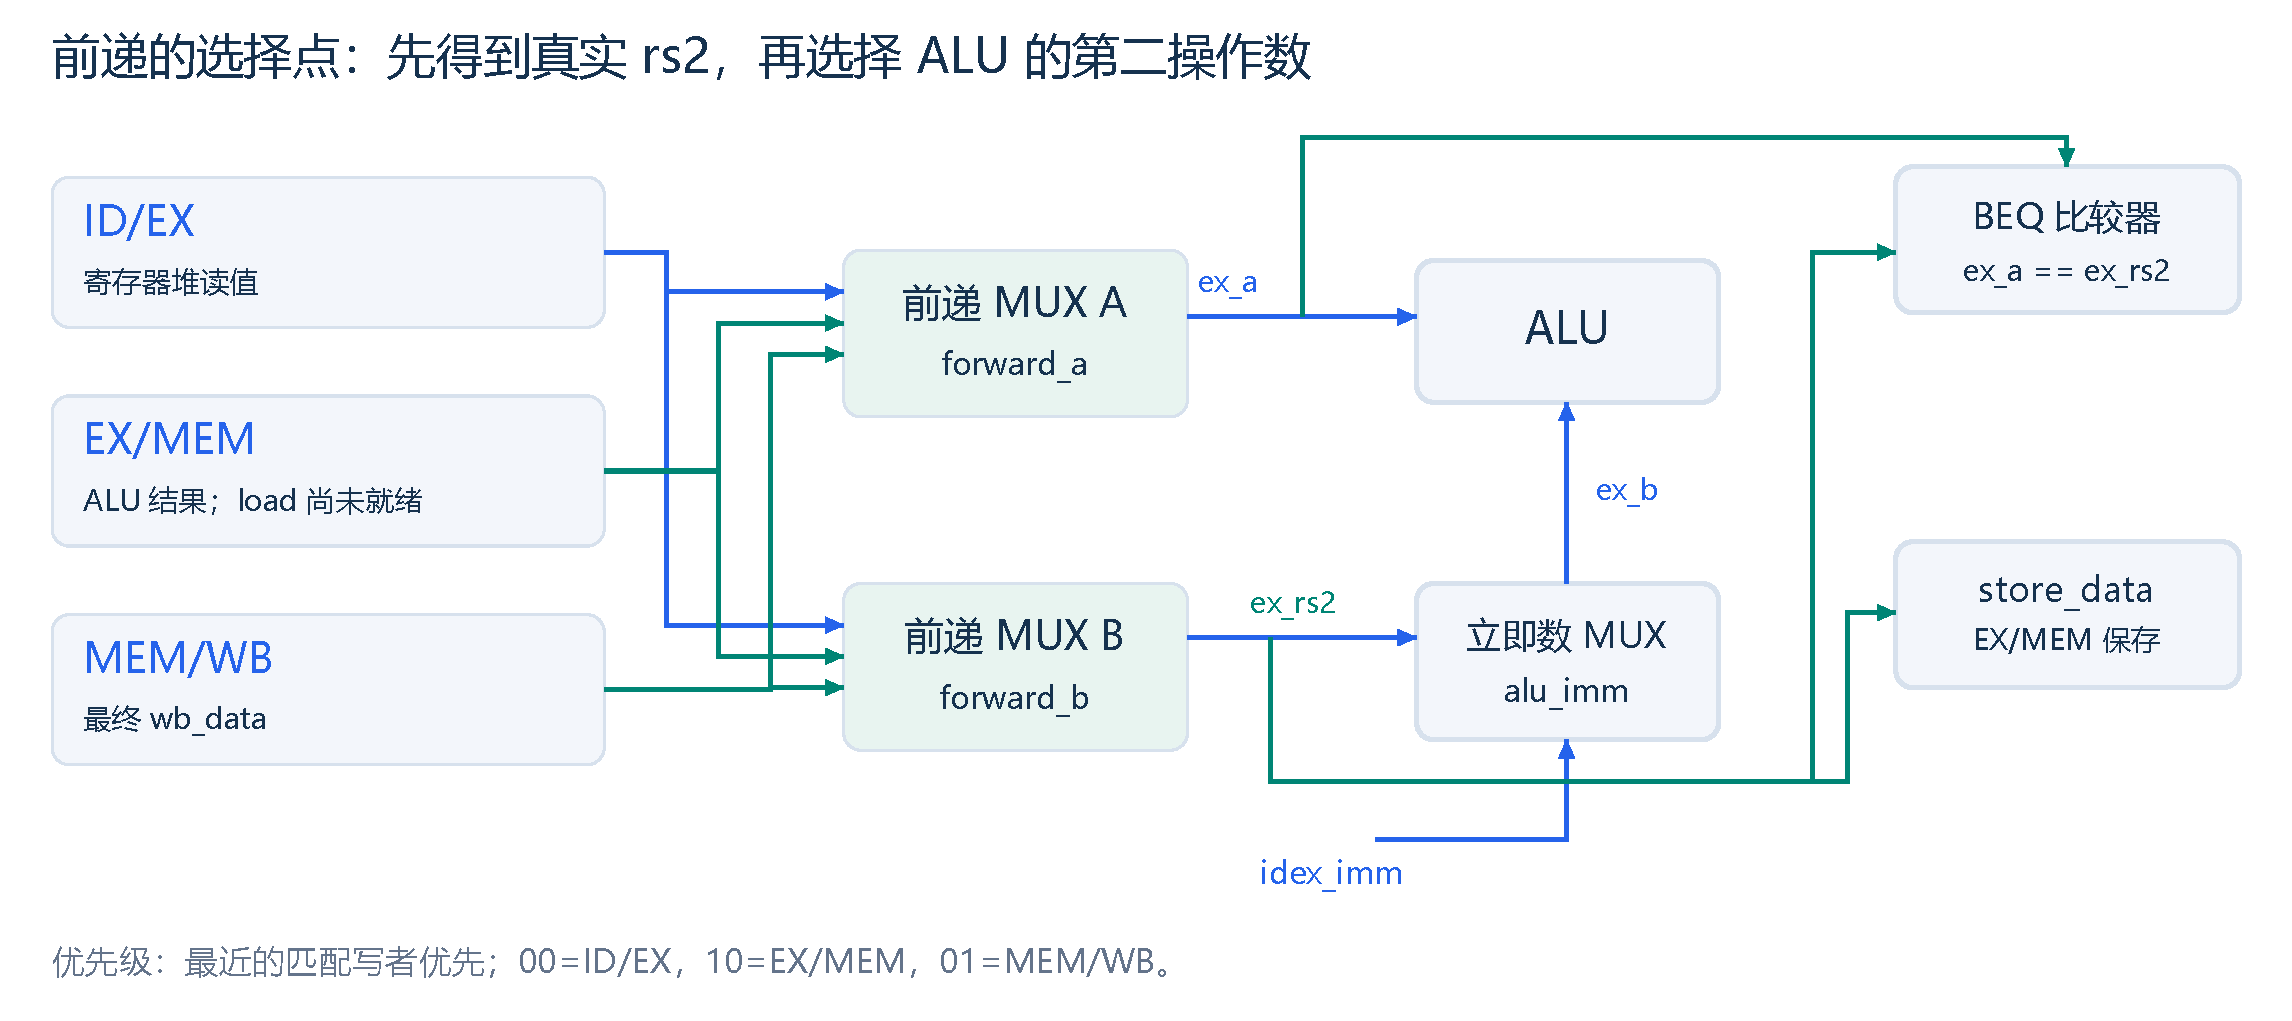
\includegraphics[width=\linewidth]{figures/05-hazard/forward-paths}
\caption{两路源操作数前递及其使用者。store 的写数据与 ALU 的立即数输入是不同路径。}
\label{fig:ch4-forward}
\end{figure}

执行级需要两个真实源值：\texttt{ex\_a} 和 \texttt{ex\_rs2}。
前递网络在 ID/EX 保存的读值、EX/MEM 的 ALU 结果和 MEM/WB 的最终写回值之间选择。
之后 ALU 第二输入还要经过立即数选择器，形成 \texttt{ex\_b}。
这两个选择步骤不能合并为“B 输入一定来自 rs2”：ADDI、LW 和 SW 的地址计算都需要立即数。

\par\noindent\begin{minipage}{\linewidth}\vspace{8pt}
\lstinputlisting[language=Verilog,caption={操作数前递、ALU 输入选择与分支比较},label={lst:ch4-operands}]{code/04-pipeline/listings/ex-operands.v}
\end{minipage}\par

对 \texttt{sw x3, 0(x0)} 来说，\texttt{ex\_a} 是地址基址，\texttt{ex\_b} 是立即数 0，
\texttt{ex\_rs2} 才是即将写入内存的数据。若把未经前递的 \texttt{idex\_rv2} 送进 EX/MEM，
即使 ALU 前递已经正确，紧邻生产者的 store 仍会写旧值。
BEQ 则必须用前递后的两个真实源值比较，不能拿未修正的 ID/EX 读值作判断。

\subsection{比较寄存器号还不够：必须比较有效性、写意图与年龄}

前递条件至少包含以下信息：消费者有效且确实使用该源寄存器；
生产者有效且会写寄存器；目的寄存器不是 x0；生产者目的号等于消费者源号；
以及该生产者的结果已经就绪。
本例控制编码为 \texttt{00=ID/EX}、\texttt{10=EX/MEM}、\texttt{01=MEM/WB}。
编码只是 MUX 选择约定，没有固定的行业含义，图、代码和波形一致即可。

\par\noindent\begin{minipage}{\linewidth}\vspace{8pt}
\lstinputlisting[language=Verilog,caption={带最近写者优先级的前递控制器}]{code/04-pipeline/forward_unit.v}
\end{minipage}\par

\paragraph{为什么 EX/MEM 优先？}
例如 \texttt{addi x1,x0,1}、\texttt{addi x1,x1,2}、\texttt{add x2,x1,x1}。
当第三条进入 EX，第一条在 WB，第二条在 MEM，两个阶段都声称可以给 x1 提供结果。
消费者需要程序顺序中最近一次对 x1 的写入，也就是第二条生成的 3，而不是第一条生成的 1。
代码用互斥的 \texttt{if / else if} 实现这种优先级，测试案例 \texttt{priority} 验证两路均选择 \texttt{10}，最终 x2=6。

\paragraph{为什么 EX/MEM 中的 load 不能前递？}
本例在 EX/MEM 的 \texttt{result} 中保存 load 的有效地址，真正载入值尚未写入 MEM/WB。
如果仅看到 \texttt{reg\_write=1} 就把 \texttt{exmem\_result} 前递，消费者拿到的是地址，不是内存数据。
因此 EX/MEM 的 load 必须禁止作为这里的数据源。

更隐蔽的问题是：较新的 EX/MEM load 与较老的 MEM/WB ALU 指令恰好写同一个寄存器。
不能因为新 load 尚未就绪，就退而使用老 ALU 的值。
本例先判断最近写者是否匹配，再判断它是否可以提供结果；若最近匹配者是 load，选择器不向老写者回退。
正确的数据就绪问题由前端暂停解决，测试平台还检查消费者不能提前进入这种 EX 状态。
\texttt{load\_overwrites\_alu} 专门覆盖了这种情况。

\paragraph{x0 不是一个需要等待的生产者。}
任何向 x0 的寄存器写入都被丢弃；任何读 x0 的结果都必须为零。
因此目的为 x0 的指令不应触发寄存器数据相关。
但是 \texttt{lw x0,0(x1)} 仍然是一条访存指令，不能因为丢弃寄存器结果就取消访存本身；
在完整实现中，相应的异常及副作用语义仍需保留\cite{ch4-rv32i}。
本例不实现异常，但 \texttt{dmem\_read} 不因目的为 x0 而被撤销。

\subsection{先用连续的 ALU 指令验证前递}

贯穿程序在 C4 中让地址 \texttt{0x04} 的 ADD 进入 EX，生产者 ADDI 在 MEM。
两路源寄存器号都是 x1，因此 \texttt{forward\_a=10}、\texttt{forward\_b=10}，执行 \(5+5=10\)。
C5 中，地址 \texttt{0x08} 的 SUB 需要 x2 与 x1。
x2 的最近写者在 EX/MEM，x1 的写者在 MEM/WB，所以 A 选择 \texttt{10}，B 选择 \texttt{01}，得到 \(10-5=5\)。
C6 的 store 再通过 B 前递取得 x3=5，C7 的上升沿将它写入地址 0。

这三拍说明前递不是修改寄存器堆的第二个写口，而是临时修正使用端看到的数据。
生产者仍按原路径到 WB，消费者也不需要重新译码。
前递有硬件成本：更多比较器、选择器与较长的组合路径，可能影响时钟周期。
“减少暂停”与“提高主频”是不同指标，不能只看 CPI 就断言总运行时间一定缩短。

\subsection{Load-Use：为什么前递仍然救不了相邻的一拍}

观察贯穿程序中的 \texttt{lw x4,0(x0)} 与 \texttt{add x5,x4,x2}。
C7 时，load 在 EX 计算地址，消费者在 ID。若不暂停，C8 时消费者就要在 EX 使用 x4，
而 load 同期才在 MEM 读出数据。
本例没有设计“MEM 组合读结果直接绕回同周期 EX”的长路径，故不能满足这个使用时刻。
暂停一拍后，C9 的消费者在 EX，load 数据已经保存到 MEM/WB，就能按普通 WB 前递处理。

检测放在 ID/EX 边界两侧：ID 中的消费者源号，与 EX 中 load 的目的号比较。
式中的 use 位避免把立即数字段误认为源号：
\begin{align*}
\mathrm{loadUse}={}&D_{\mathrm{valid}}\land E_{\mathrm{valid}}
 \land E_{\mathrm{memRead}}\land(E_{rd}\ne0)\\
 &\land\big[(D_{\mathrm{use1}}\land D_{rs1}=E_{rd})
 \lor(D_{\mathrm{use2}}\land D_{rs2}=E_{rd})\big].
\end{align*}

\par\noindent\begin{minipage}{\linewidth}\vspace{8pt}
\lstinputlisting[language=Verilog,caption={Load-Use 检测与前端控制}]{code/04-pipeline/hazard_unit.v}
\end{minipage}\par

\paragraph{暂停时，分别操作三个边界。}
第一，PC 保持，避免继续消耗尚未进入流水线的指令；第二，IF/ID 保持，让消费者继续留在 ID；
第三，ID/EX 在边沿置为无效，给 EX 注入一个空泡。
EX/MEM 与 MEM/WB 正常推进，让造成相关的 load 继续完成。
若连 ID/EX 一起保持，load 会一直待在 EX，相关条件也一直成立，流水线便可能无法前进。
若只保持 PC 而不保持 IF/ID，消费者又可能被覆盖或重复注入。

\begin{figure}[htbp]
\centering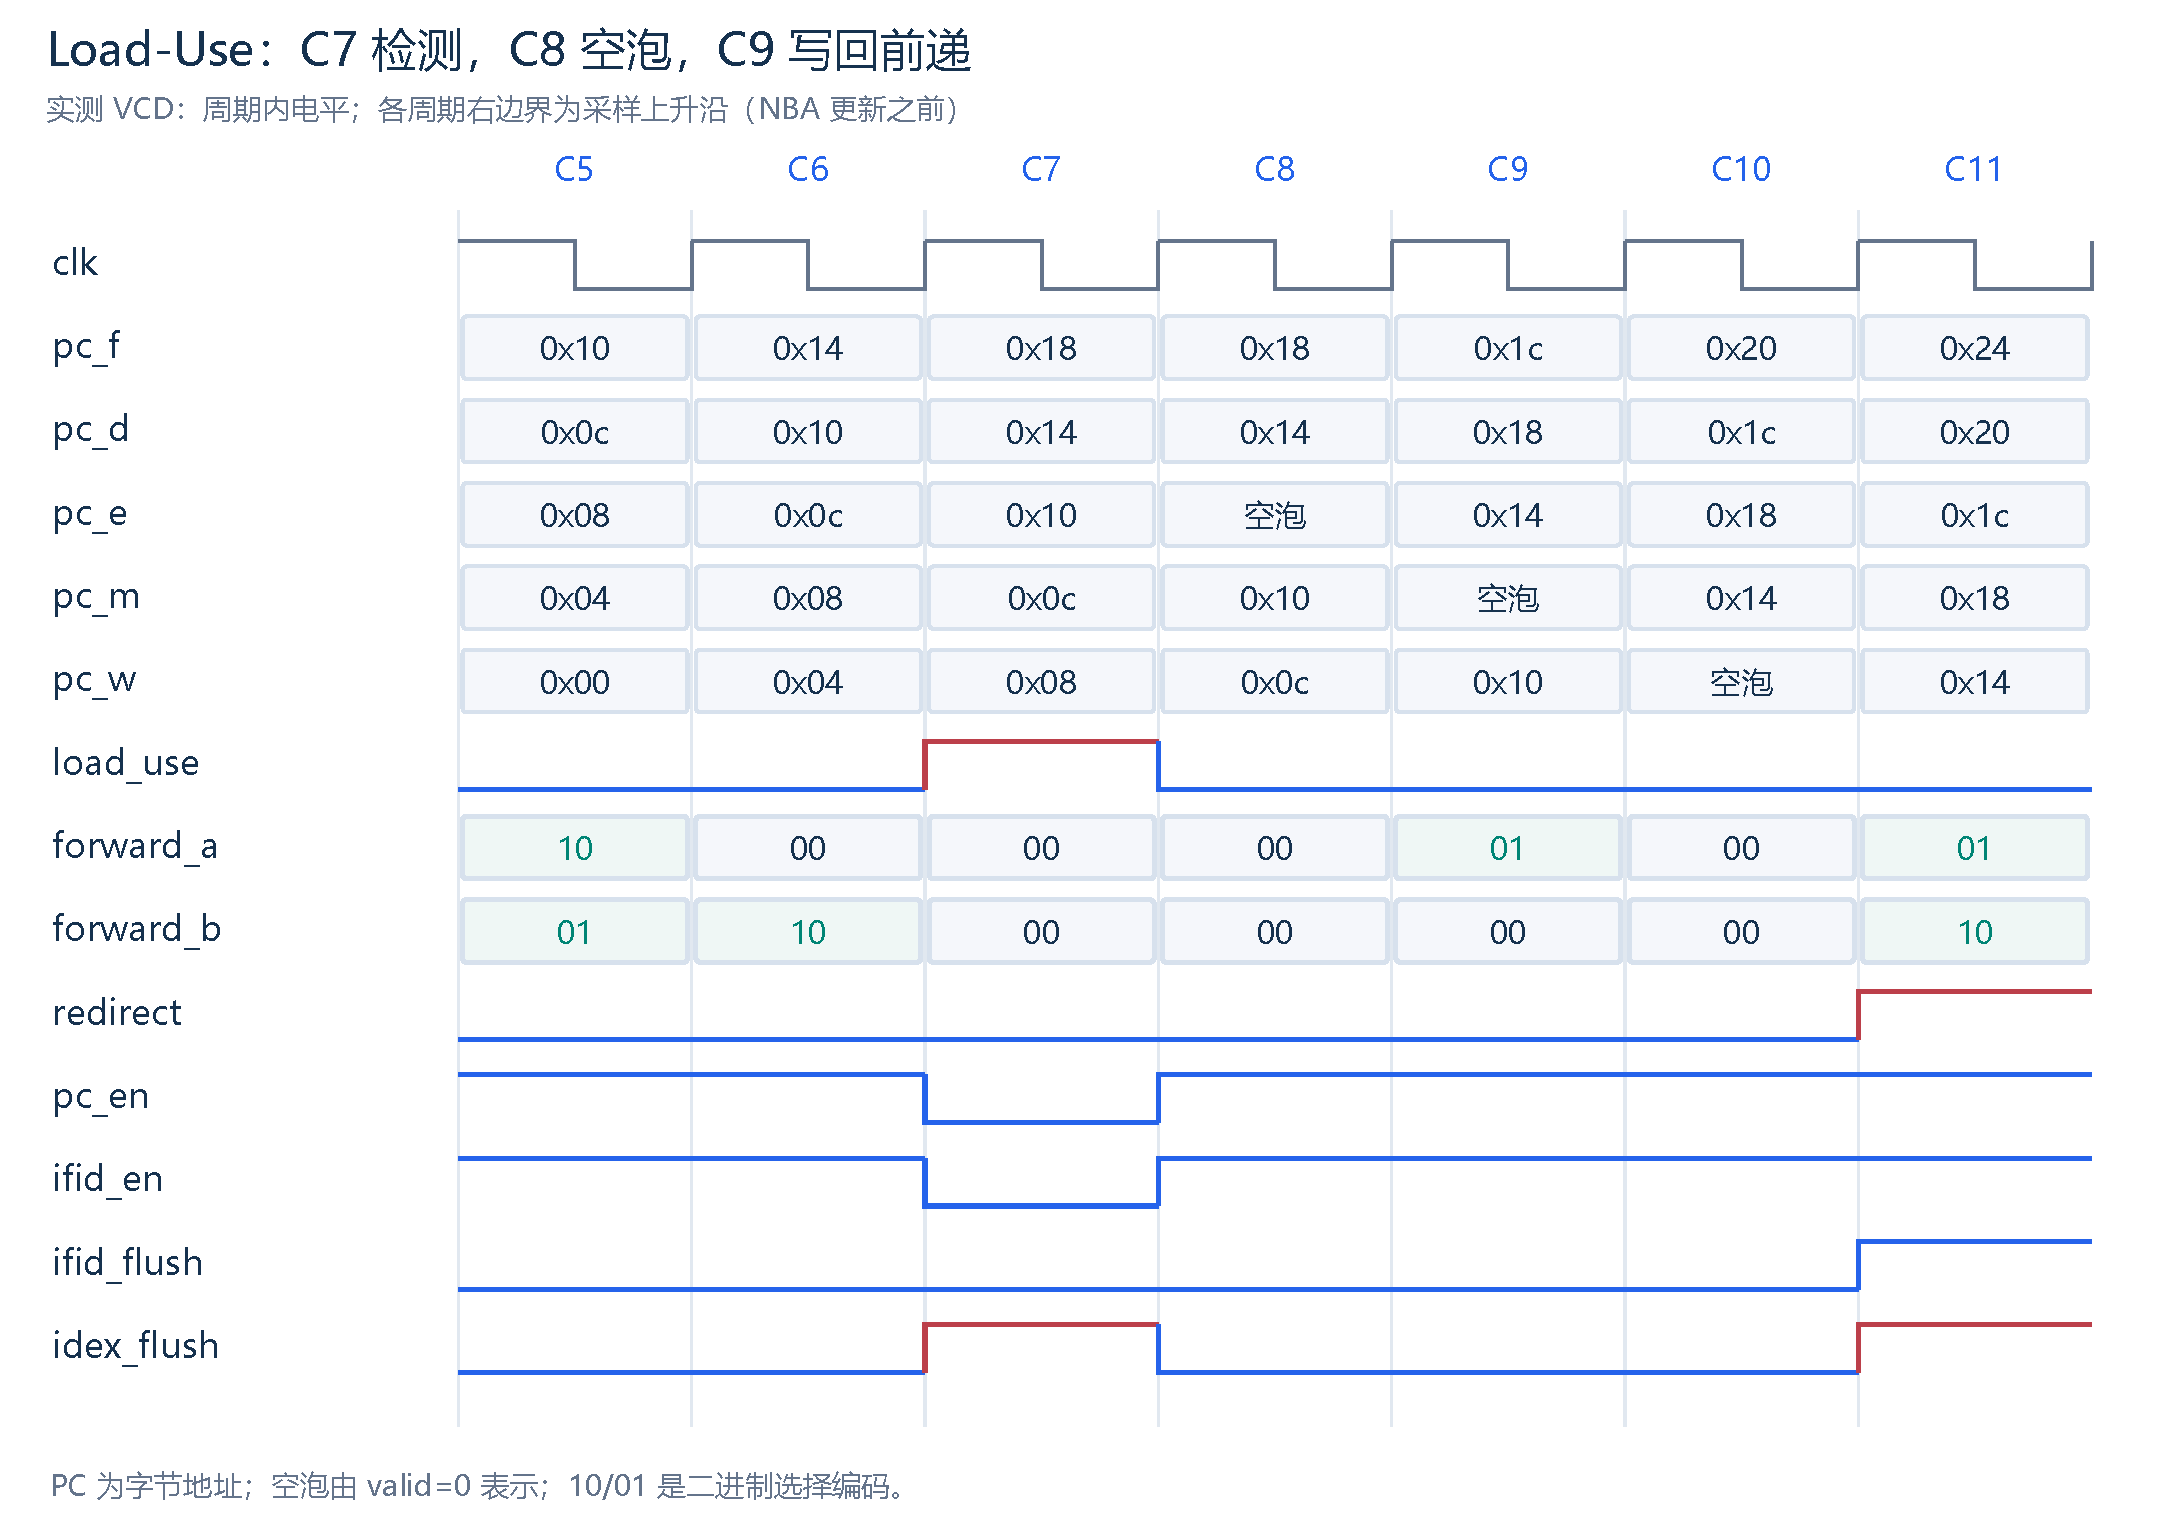
\includegraphics[width=\linewidth]{figures/05-hazard/wave-load-use}
\caption{实际仿真中的 Load-Use 控制波形。总线只显示有效 PC；有效位为零时标为空泡。}
\label{fig:ch4-load-wave}
\end{figure}

\begin{table}[htbp]
\centering\small
\caption{Load-Use 的三个关键周期}\label{tab:ch4-load-cycles}
\begin{tabularx}{\linewidth}{p{.10\linewidth}p{.30\linewidth}Y}
\toprule
周期 & 边沿前所在位置 & 本周期控制与边沿后的变化 \\\midrule
C7 & LW 在 EX，ADD 在 ID & load\_use=1；pc\_en=0、ifid\_en=0、idex\_flush=1；load 继续到 MEM。\\
C8 & LW 在 MEM，EX 为空泡，ADD 仍在 ID & load\_use=0；前端恢复推进，边沿后 ADD 进入 EX，载入值进入 MEM/WB。\\
C9 & LW 在 WB，ADD 在 EX & forward\_a=01；ADD 使用 x4=5 与 x2=10，得到 15。\\
\bottomrule
\end{tabularx}
\end{table}

\paragraph{一拍暂停是本例条件下的结论。}
本例把 store 数据也在 EX 取齐并保存在 EX/MEM，所以相邻 \texttt{lw x1,...; sw x1,...} 也停一拍。
如果另加 WB 到 MEM 的 store 写数据旁路，那么只依赖 store 数据、而不依赖其地址基址的情况可能不必停。
这种优化需要重新区分源操作数的使用级，不能简单把 SW 的 use2 改成 0。
同理，若存储器增加等待周期，就需要持续保持相关状态，当前的一拍控制不能直接复用。

\subsection{暂停与冲刷解决的是不同问题}

暂停表示“这条指令仍然要执行，只是现在不能前进”；冲刷表示“这条指令不应再执行”。
在本例的 taken BEQ 中，决定分支的指令位于 EX，IF 与 ID 已经有两条按顺序 PC 取来的年轻指令。
如果分支成立，它们属于错误路径，必须在下一个边沿失效。
因此重定向同时作用于 PC、IF/ID 和 ID/EX；更老的 MEM、WB 指令继续完成。

\begin{table}[htbp]
\centering\small
\caption{控制优先级与各流水边界动作}\label{tab:ch4-controls}
\begin{tabularx}{\linewidth}{p{.21\linewidth}p{.17\linewidth}p{.17\linewidth}p{.17\linewidth}Y}
\toprule
条件（自上而下） & PC & IF/ID & ID/EX & EX/MEM、MEM/WB \\\midrule
同步复位 & 置为 0 & valid=0 & valid=0 & valid=0\\
redirect=1 & 分支目标 & valid=0 & valid=0 & 旧指令推进\\
load\_use=1 & 保持 & 保持 & valid=0 & 旧指令推进\\
正常周期 & PC+4 & 接收 IF & 接收 ID & 旧指令推进\\
\bottomrule
\end{tabularx}
\end{table}

代码中 IF/ID 的 flush 判断位于 enable 之前，所以即使使能关闭，冲刷也能取消其中的旧指令。
\texttt{pc\_en = redirect || !load\_use} 则保证重定向不会被普通暂停屏蔽。
在当前单发射实现中，同一条 EX 指令不可能既是 load 又是 BEQ，二者不会同时触发；
仍然明确优先级，有助于以后加入其他暂停来源时保持控制语义清晰。

\paragraph{为什么只清 IF/ID 不够？}
在分支决定的边沿，原 ID 中的错误路径指令正准备进入 ID/EX。
只清 IF/ID，会让该指令同时进入 EX，后续仍可能写寄存器或内存。
本例同时使 IF/ID 和 ID/EX 失效，取消的正好是 EX 分支之后的两条年轻指令。
这里没有分支延迟槽；RISC-V 软件也不能把被取消的指令当成必执行指令。

\subsection{从真实波形检查一次分支冲刷}

C11 时，地址 \texttt{0x1c} 的 BEQ 在 EX。它读取的 x5 来自 MEM/WB，x6 来自 EX/MEM，
所以两路前递选择分别为 \texttt{01} 和 \texttt{10}。
比较值均为 15，\texttt{redirect=1}，目标为 \(\mathtt{0x1c}+12=\mathtt{0x28}\)。
同一周期，ID 中是地址 \texttt{0x20} 的 ADDI，IF 中是地址 \texttt{0x24} 的 SW。
它们在边沿被取消。

\begin{figure}[htbp]
\centering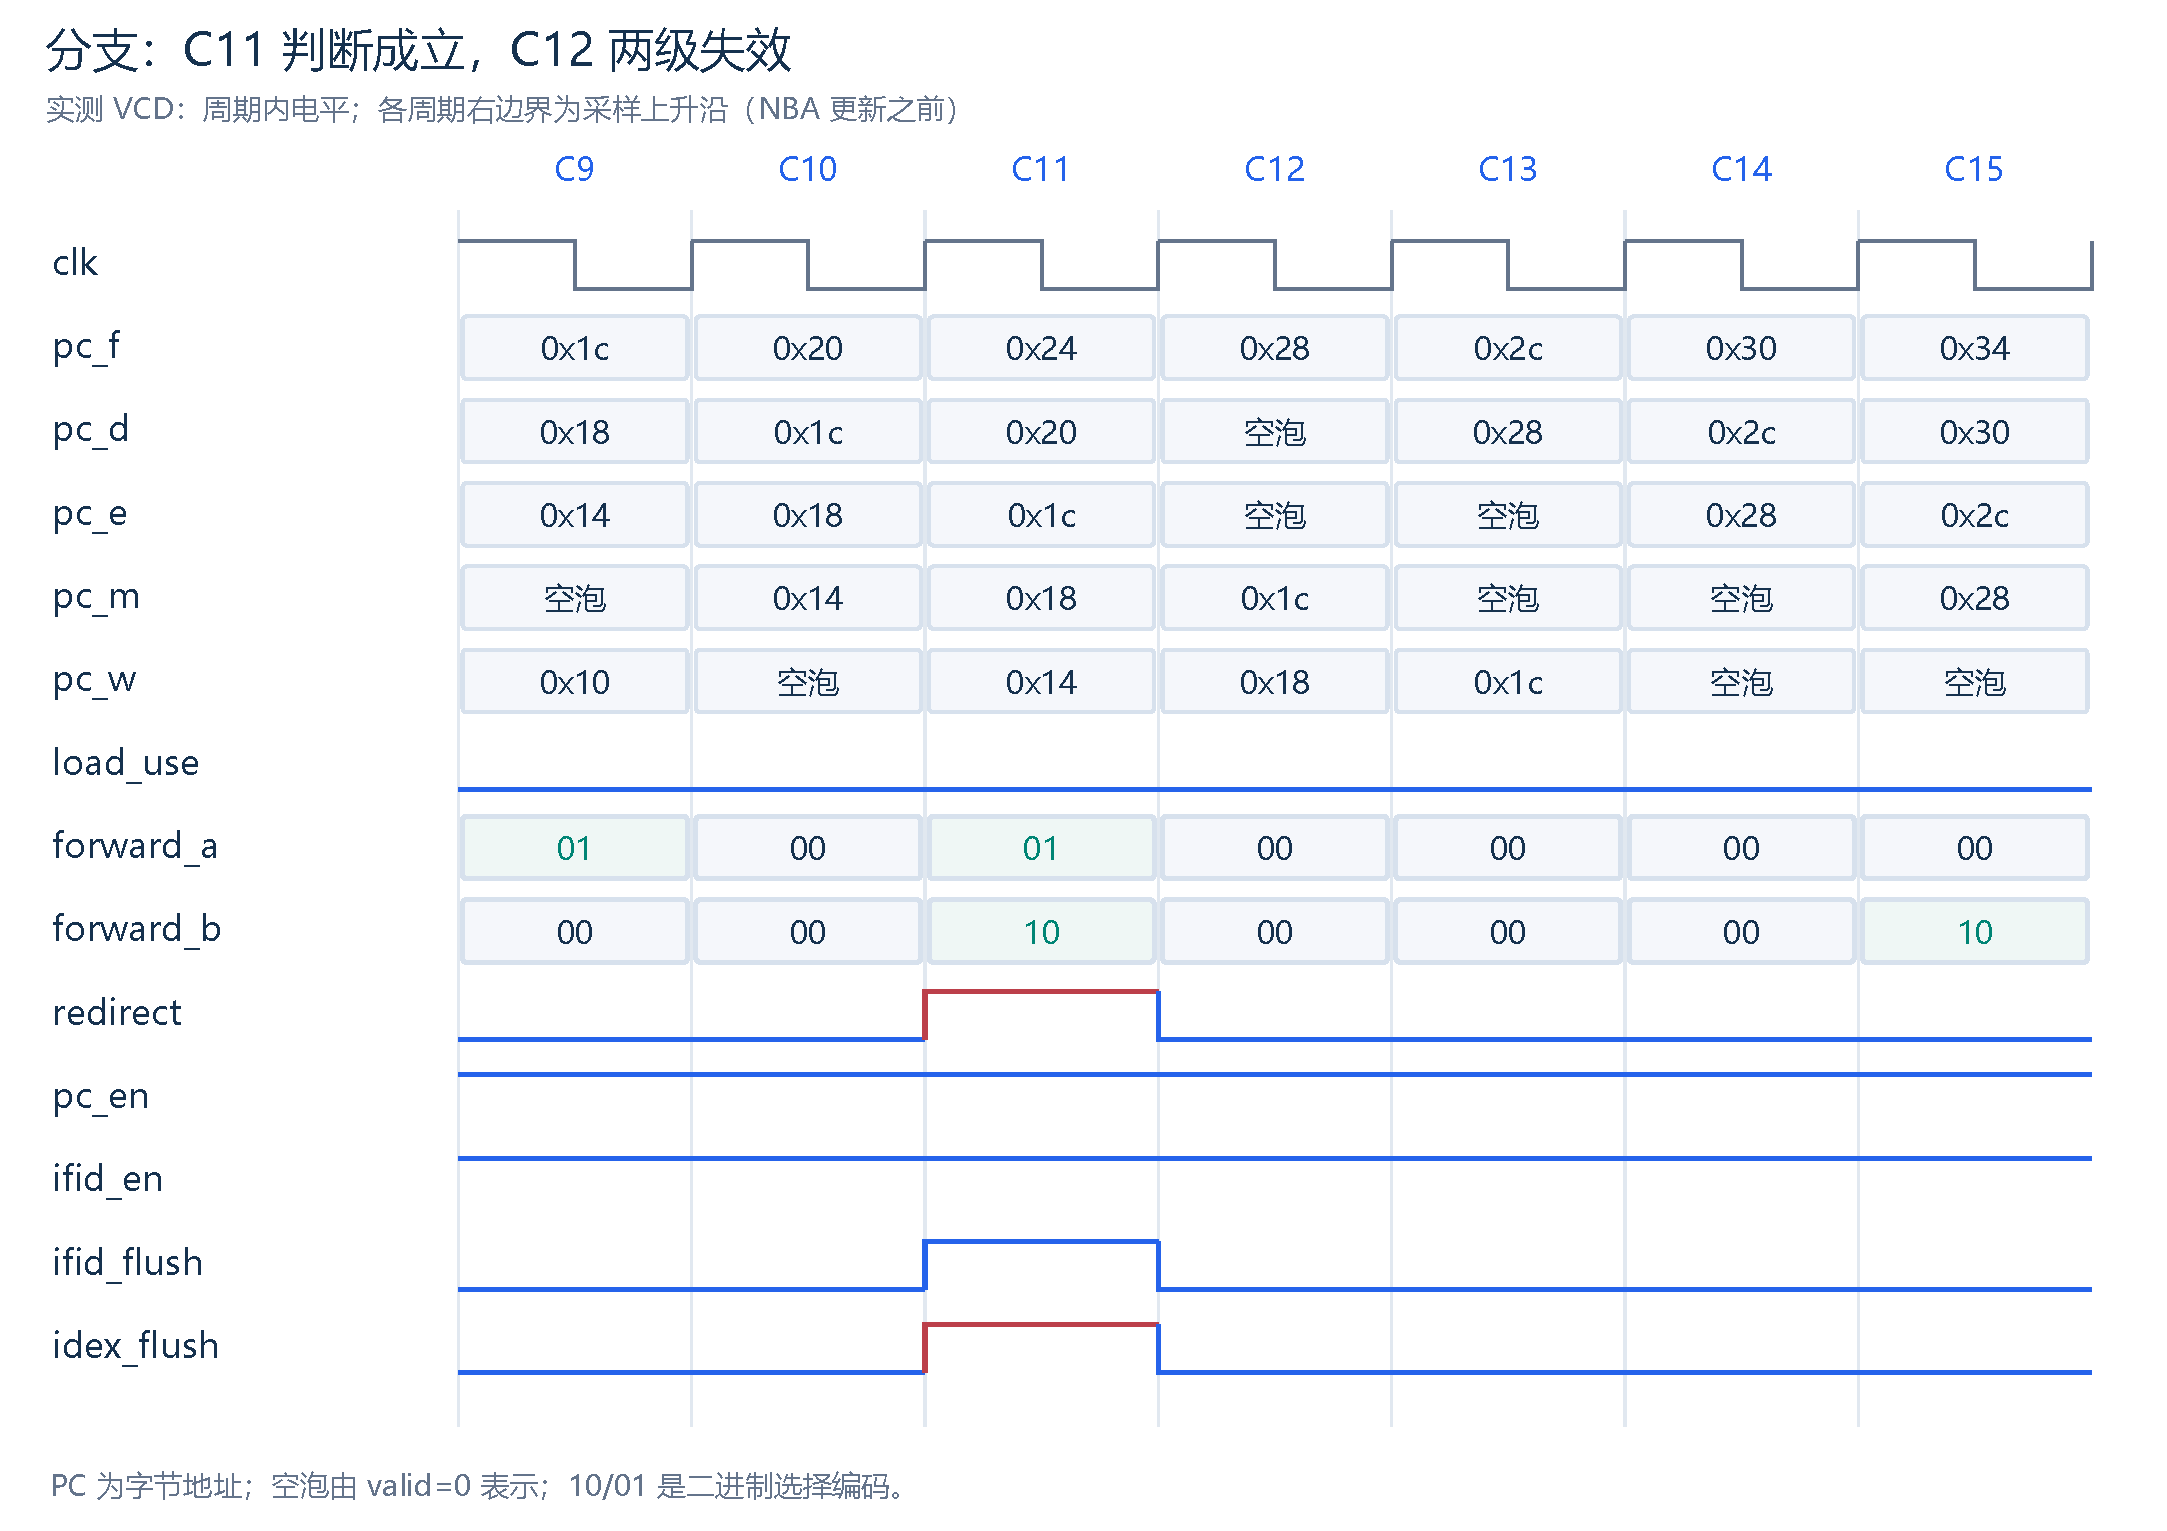
\includegraphics[width=\linewidth]{figures/05-hazard/wave-branch}
\caption{实际仿真中的分支冲刷。C12 的 IF 已在目标地址，ID 与 EX 同时为空泡。}
\label{fig:ch4-branch-wave}
\end{figure}

C12 取到正确目标，C13 目标进入 ID，C14 进入 EX。
BEQ 自己仍可沿 MEM、WB 传播，但它的寄存器写与存储器写控制均为零。
被冲刷的 ADDI 不会写 x7，被冲刷的 SW 不会覆盖地址 4。
最终检查 x7=0 和 memory[4]=32，既验证目标地址，又验证错误路径没有造成副作用。

\begin{figure}[htbp]
\centering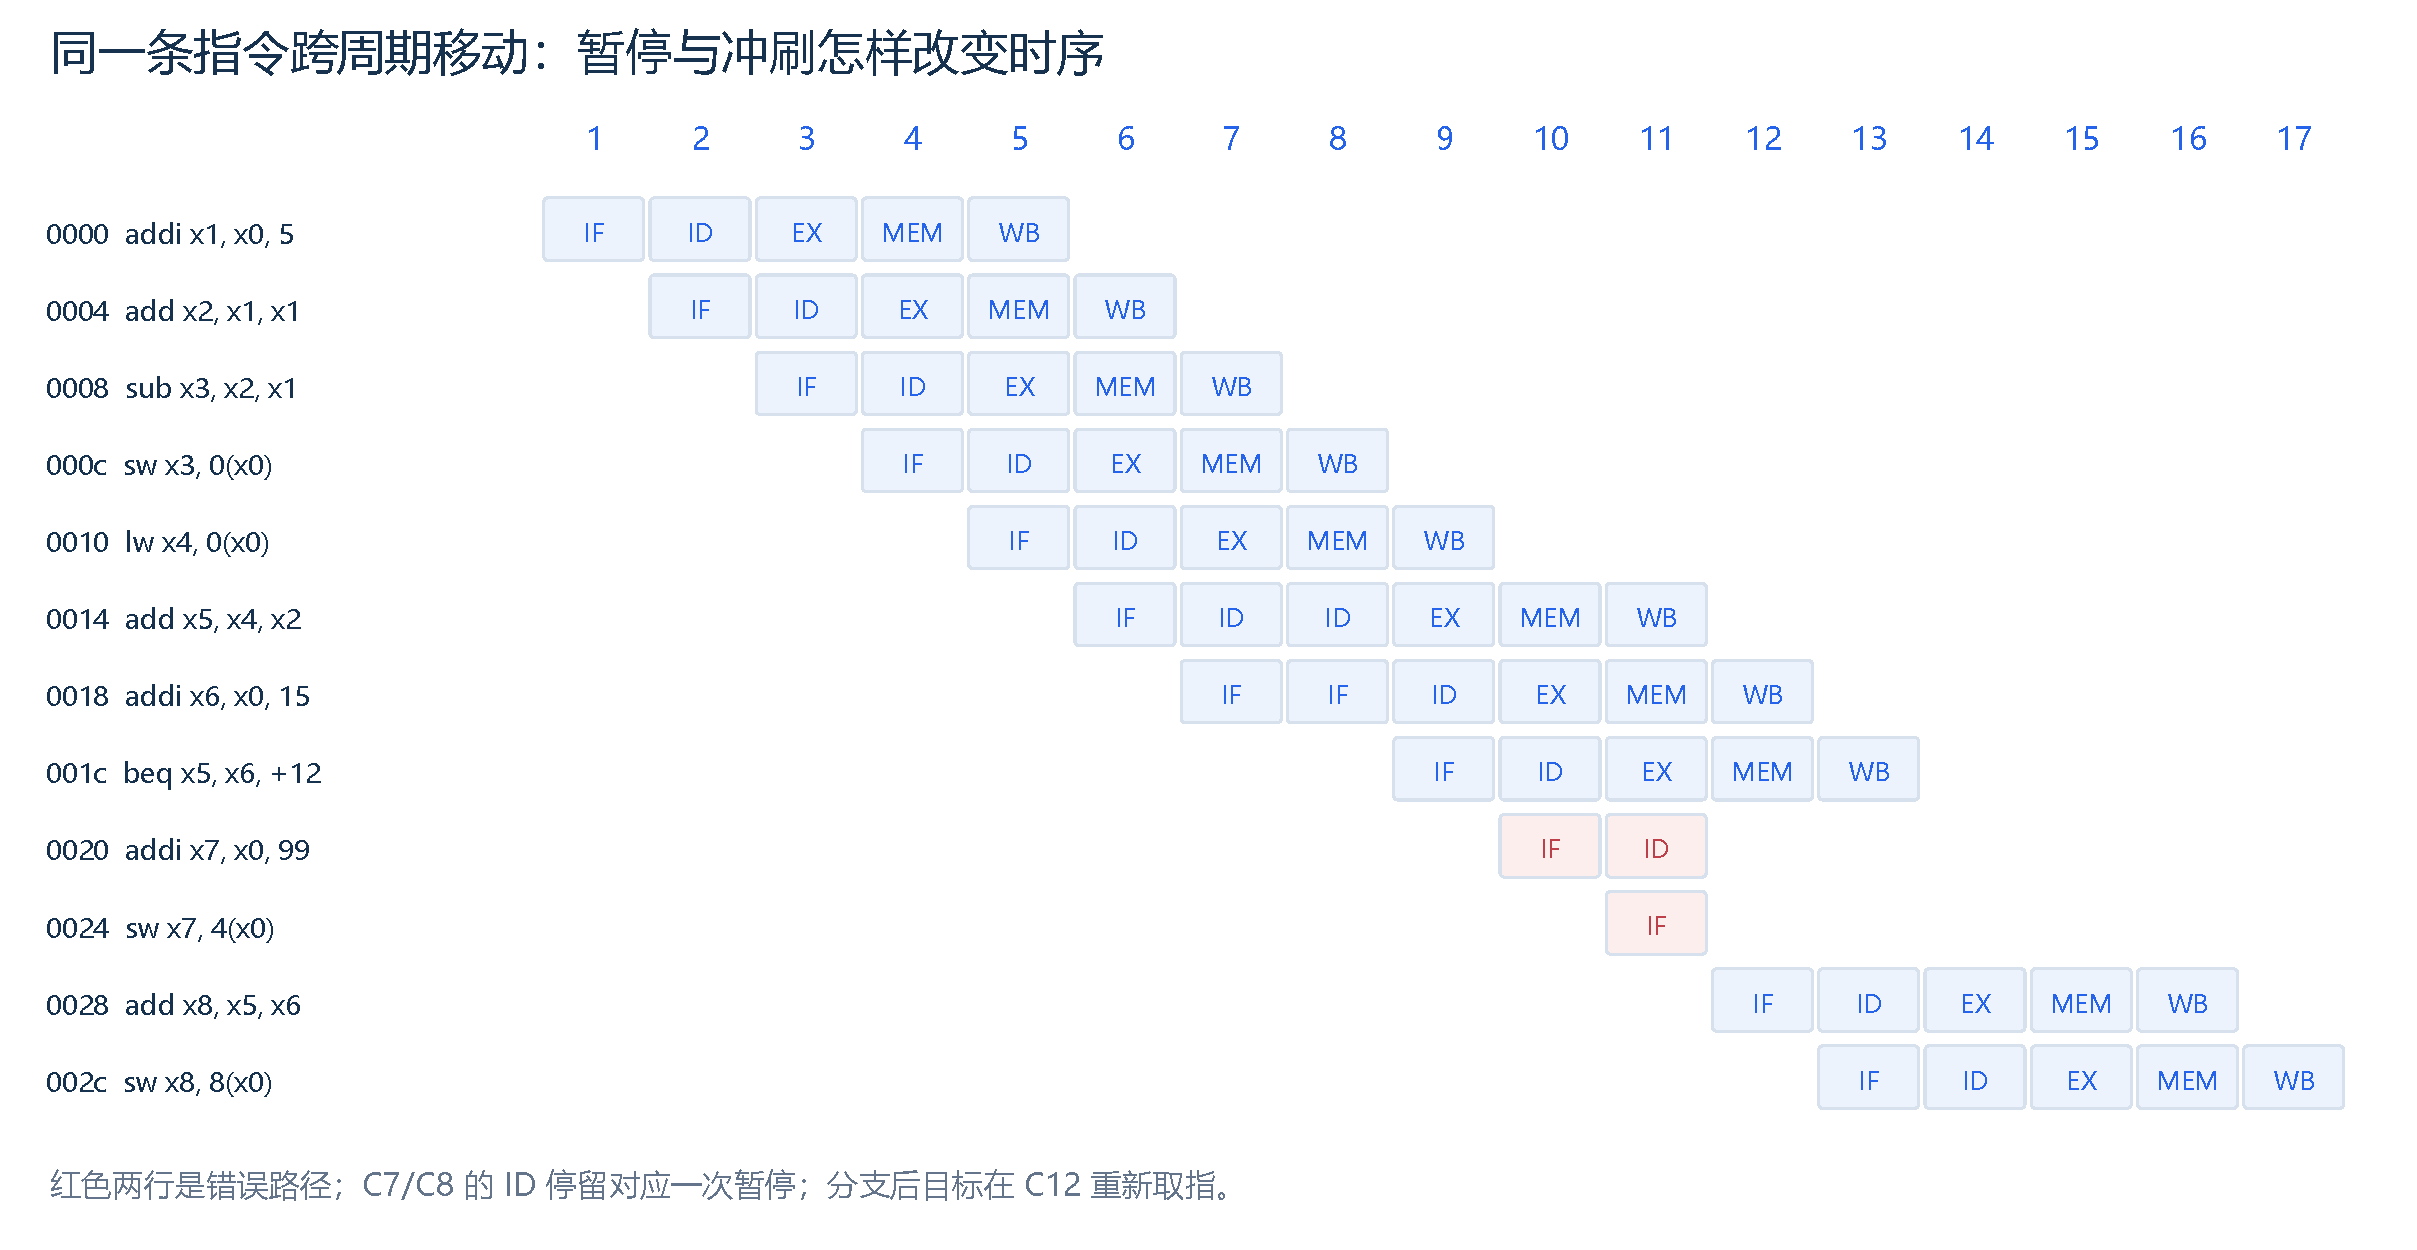
\includegraphics[width=\linewidth]{figures/05-hazard/cycle-table}
\caption{贯穿程序的实际流水时序。横轴为周期，红色标出被取消的路径。}
\label{fig:ch4-cycle-table}
\end{figure}

这里 taken branch 的代价是失去两条年轻指令占据的前端机会。
若把分支判断提前到 ID，冲刷范围可以变化，但比较器也需要更早拿到源值，前递和暂停都要重新设计。
若使用分支预测，则“成立”与“错误预测”更不再是一回事。
本例只有固定的顺序取指策略，不把它称为实现了完整分支预测器。

\subsection{怎样把“看起来对”变成可复现的验证}

波形适合解释时间关系，自动判定适合防止漏看。
本实验同时检查架构结果和周期约束。
Python 参考模型独立解码实际机器码，顺序执行支持的指令，产生期望的寄存器写入序列和存储器写入序列。
测试平台只在真实写使能有效的边沿记录 RTL 事件，再按事件类别逐项比较 PC、目的对象和数据。
store 在 MEM 发生、寄存器写在 WB 发生，所以这两类事件分别比较顺序，避免把不同观测级的交错误当成程序提交顺序。

测试平台还检查更具体的时序性质：上一拍发生 load-use 后，PC 和 IF/ID 必须保持，ID/EX 必须为空，
原 EX load 必须进入 MEM；上一拍重定向后，PC 必须为目标，两组年轻流水寄存器必须失效；
消费者不能在较新的匹配 load 尚处 MEM 时提前使用旧值；x0 不能被修改。
这些检查能在结果偶然正确时仍发现控制错误。

\begin{table}[htbp]
\centering\small
\caption{2026-10-23 使用 Icarus Verilog 执行的验证结果}\label{tab:ch4-tests}
\begin{tabularx}{\linewidth}{p{.30\linewidth}Yrr}
\toprule
案例 & 重点 & 暂停 & 重定向 \\\midrule
walkthrough & 两路前递、store、load-use、错误路径取消 &1&1\\
priority & 两个未完成写者同时匹配，选择最近写者 &0&0\\
wb\_id & WB 与 ID 同拍访问同一寄存器 &0&0\\
x0\_false\_dependency & x0、立即数字段造成的假相关 &0&0\\
load\_store & load 到 store 数据及地址相关 &2&0\\
load\_overwrites\_alu & 新 load 覆盖旧 ALU 写者 &1&0\\
load\_branch & load 到分支，成立与不成立两种结果 &1&1\\
random\_160 & 固定种子 20261023，160 条混合指令 &6&0\\
\bottomrule
\end{tabularx}
\end{table}

八组测试全部通过，覆盖 197 条输入指令，其中有错误路径指令不实际执行。
随机组包含 ADD、SUB、ADDI、LW、SW，限制地址对齐且在数组范围内，没有随机分支或异常。
这是一组针对本节机制的教学验证，不等同于完整 ISA 测试、形式化证明或 FPGA 时序签核。
复现时应以本机新生成的 \texttt{summary.json} 和日志为准。

\paragraph{为什么要说明波形的采样时刻？}
测试平台在上升沿的活动区读取边沿前的值，随后 DUT 的非阻塞赋值更新各流水寄存器。
因此本文的 C7 表示“C7 结束的上升沿之前的状态”，暂停产生的空泡在下一列 C8 可见。
若在波形工具中把游标放到该边沿之后，就会看到更新后的 C8 状态。
二者没有矛盾，只是采样定义不同。

\texttt{generate\_assets.py} 解析原始 \texttt{wave.vcd}，
在每个有效上升沿之前采样，并逐拍核对八个控制信号与 \texttt{trace.csv}。
两张控制波形图由这些已核对的数据生成，未用手填的理想时序替代实际仿真。
图中 PC 总线只在对应有效位为 1 时显示，否则标作空泡。
原始 VCD 保留了所有信号，读者仍可检查被图形隐藏的无效载荷。

\paragraph{建议的观察步骤。}
先打开 \texttt{walkthrough/wave.vcd}，加入 clk、rst、各级 valid 与 PC；
再加入 load\_use、forward\_a/b、redirect、pc\_en、ifid\_en 和两路 flush；
最后加入 ex\_a、ex\_rs2、wb\_we、wb\_data、dmem\_write。
从 C4、C7、C11 三处开始检查，分别回答“值从哪来”“哪一级保持”“哪些指令被取消”。
只看最终寄存器值，无法解释这些周期行为；只看几根控制线，也无法证明最终程序效果正确。

\subsection{动手修改：让错误暴露在正确的测试里}

可以复制实验目录再做以下练习；每次只改一个机制，先预测哪个案例失败，再运行验证。
修改实验副本时保留原始通过版本，方便对照。
\begin{enumerate}
\item 交换前递优先级。预测 \texttt{priority} 中 x2 的错误结果，并在 EX 两个匹配写者同时存在时观察选择信号。
\item 移除 \texttt{d\_uses\_rs2} 条件。观察 \texttt{x0\_false\_dependency} 中立即数 5 是否触发多余暂停；此类错误可能不改变计算结果，但会改变周期计数。
\item 把 load-use 时的 ID/EX 清空改为保持。解释为什么 load 无法离开相关位置；仿真应由时序约束或事件数量检查暴露问题。
\item 把 store 数据改接未经前递的 ID/EX 读值。先检查贯穿案例地址 0 的写数据，再解释为何 ALU 的有效地址可能仍然正确。
\item 分支成立时只清 IF/ID。观察地址 \texttt{0x20} 的错误路径指令是否继续进入 EX，是否最终写入 x7。
\end{enumerate}

\paragraph{思考题参考线索。}
最近的写者代表程序顺序中消费者应读到的版本；立即数字段不是源寄存器；
等待的消费者应停住，而生产者必须前进；store 地址与 store 数据是两条独立路径；
在分支决定的边沿，ID 正准备把年轻指令传给 EX。
用这些因果关系解释失败，比仅把代码改回去更能建立硬件思维。

\KeyPoint{从理论到 RTL 的完整检查链}{
先标出指令的生产者与消费者，再标出结果就绪级与使用级；把这些条件写成寄存器号比较、MUX 选择、使能与有效位；
最后同时检查逐拍波形和架构结果。前递修正数据来源，暂停推迟使用时刻，冲刷取消不该发生的操作。}
